\documentclass[12pt]{article}
\usepackage{graphicx}
\usepackage{layout}
\usepackage[margin=1in]{geometry}
\usepackage{setspace}
\usepackage{float}

\doublespacing

\begin{document}

\begin{flushleft}
	Arjun Phull\\
	Millhouse\\
	ISTA 450\\
	13 December 2023
\end{flushleft}

\begin{center}
	``Take that, NYT Games!" Applying AI Search Algorithms to 9x9 Sudoku
\end{center}
\textbf{Introduction}

	I have a love-hate relationship with the New York Times' Games app. Wordle is a fan favorite, the Mini crossword is always a good time, and the Connections and I go way, way back. But nothing humbles me more than the daily Sudoku puzzle. Every time, I click on the hard puzzle. Every time, I think I'm getting somewhere. And every time, I get stuck. I thought to myself: there has got to be a faster way to solve these puzzles. I was fed up with the New York Times constantly embarrassing me, day in and day out. So, I got to work.

	Here's a quick refresher on the rules of Sudoku: each game is played on a 9x9 board, which itself is subdivided into nine 3x3 subgrids. The board begins with some pre-filled cells. These are called 'givens', the amount of which determines how difficult the puzzle is. More givens make for an easier puzzle, and vice versa. The goal of the game is to fill in each blank square with a digit from 1 to 9. Easy enough, right? Well, there are some rules that determine which numbers can go where. Within any single row, column, or subgrid, there can be exactly one occurrence of each digit 1 through 9.
	
	At first glance, the game of Sudoku may just seem like a brainteaser. But upon closer inspection, the task becomes clearer: one must choose values for each empty cell that satisfy certain row, column, and subgrid rules, or constraints. Therefore, Sudoku is nothing but a constraint satisfaction problem. And we have ways of solving constraint satisfaction problems! In this project, I've implemented a Python class that handles a game of Sudoku. I've then implemented three constraint satisfaction problem solving algorithms: local search, general backtracking search, and backtracking search with constraint propagation. My goal was to determine which of the three algorithms is optimal for solving even the mightiest of Sudoku puzzles.\\\\
\textbf{Conceptual Overview}

	Let's first talk about the concepts at hand. A constraint satisfaction problem, or CSP, has three components: a set of variables; a set of domains, one for each variable; and a set of constraints that specify how the values of each variable can be combined (Russell and Norvig, 2009). The CSP is considered solved if each variable's value satisfies all its constraints. In the case of Sudoku, the variables are the empty cells, the domains are the digits 1 through 9, and the constraints are the row, column, and subgrid rules.
	
	Local search is an algorithm that relies on random choice to solve a CSP. The approach begins by first assigning a random value to each variable. This initial assignment often violates many of the problem's constraints. The search algorithm then changes the value of a randomly chosen variable at a time in the hopes of reducing the number of constraint violations, or conflicts. The new value that is assigned can be randomly chosen, but it is often set as the value that minimizes the total number of conflicts. The algorithm will continue to iteratively select a random variable and change its value until a solution is found or a maximum number of iterations is reached. Since the choice of variable is random, as opposed to heuristic-guided, local search is far from optimal and is not guaranteed to return a solution.
	
	Backtracking search is an algorithm that uses partial assignments, as opposed to local search's complete assignment, to find a solution. The algorithm uses depth-first search to assign values to one variable at a time. If a variable assignment causes a conflict, the algorithm backtracks, reverts that assignment, and tries another value. This algorithm is recursive, and it is guaranteed to find a solution. A general implementation of backtracking search will attempt to fill each unassigned variable in the order they appear, and it will test values across its entire domain, ignoring constraints. While this is a robust way of testing and filling values and variables, it is not the most efficient approach.
	
	Constraint propagation search is a specialized implementation of backtracking search. The algorithm structure is similar to that of general backtracking, with a few key differences. Constraint propagation search chooses each unassigned variable using the Minimum Remaining Values (MRV) heuristic---that is, the algorithm will choose the variable with the fewest possible values first. When testing values for each variable, the algorithm will only iterate over that variable's possible values. This eliminates computations, making for a faster search algorithm. However, this requires the underlying data structure (in our case, the game of Sudoku) to keep track of the possible values for each variable after each iteration.\\\\
\textbf{Python Implementation}
	
	To use these algorithms for Sudoku, I first had to implement a game of Sudoku. In Python, I implemented a class called \textit{sudokuGame}, which defines the structure and functionality of a game of 9x9 Sudoku. The class contains methods to initialize a board, get the candidates for a cell, and calculate the number of conflicts on the board, among other key functions. I then implemented each of the search algorithms, leveraging the structure of \textit{sudokuGame}.
	
	The function \textit{redactCells} is a utility function that takes a complete Sudoku board as input and redacts a specified number of values, creating a solvable Sudoku puzzle. This was useful for creating a set of test boards to use when comparing the three solving algorithms.
	
	The function \textit{\textit{minConflicts}} uses local search to find the solution to a \textit{sudokuGame}. It begins by initially assigning random values to each blank cell on the board. It then iterates over the maximum number of steps passed into the function. For each step, the algorithm counts the number of conflicts on the board. If there are no conflicts, the board is solved. Otherwise, the function assembles a list of cells that cause conflicts. It chooses a conflicting cell at random and sets its value to the value between 1 and 9 that minimizes the total number of conflicts on the board. The algorithm repeats this until a solution is found or the maximum number of iterations is reached. If the algorithm does not improve the number of conflicts after successive iterations, the search is said to have reached a plateau. At this point, each cell that was initially blank is re-randomized, and the search continues.
	
	The functions \textit{backtrackingSearch} and \textit{backtrack} use a recursive implementation of backtracking search to find the solution to a \textit{sudokuGame}. Each call selects the first empty cell on the board. The algorithm then tries to set its value to each digit 1 through 9. After each assignment, the algorithm calls \textit{backtrack} again. If the recursive call ever fails (i.e. if a variable assignment ever causes a conflict), the algorithm backtracks, reverts the assignment, and tries another value. This recursion repeats until the board is solved.
	
	The function \textit{constraintProp} integrates backtracking with constraint propagation across each variable to find the solution to a \textit{sudokuGame} quickly and efficiently. Whereas \textit{backtrack} selects the first empty cell, \textit{constraintProp} selects the empty cell with the fewest remaining values. \textit{constraintProp} leverages \textit{getCandidates}, a method within \textit{sudokuGame} that traverses the board and logs the possible values for each cell according to row, column, and subgrid constraints. When testing values to assign to the empty cell, \textit{constraintProp} only iterates over the cell's candidates. This saves time and computations in the long run. After each assignment, the algorithm calls \textit{constraintProp} again. If the recursive call ever fails, the algorithm backtracks, reverts the assignment and constraints, and tries another value. By the nature of Sudoku, as more values are filled, the remaining empty cells will have fewer and fewer candidates. This algorithm prioritizes filling in values that are more restricted than others, making it more efficient.\\\\
\textbf{Challenges in Implementation}
	
	When implementing local search, I was not sure how to handle variable assignment. I initially considered having the algorithm choose two cells at random and swap their values. I quickly realized that this would not work in the case where there was only one cell to swap. So, I then thought to have the algorithm randomly choose a variable, and then assign a random value to that variable. This approach was better and worked well for boards with only a few missing values. Mathematically, this was expected behavior. The number of possible complete assignments for a board with $n$ blank spaces is $9^n$. So, an algorithm that randomly assigns variables was bound to find the solution to a puzzle with two or three blank spaces within a few thousand iterations. However, this did not fare well for even slightly more complex puzzles. So, I implemented a greedy assignment process that assigned to each chosen cell the value that minimized total conflicts. And this worked! When I tested \textit{minConflicts}, though, the algorithm would often find a local optimum, or a set of value assignments that, individually, minimize the number of conflicts, but as a set, do not. To curb this, I added a counter variable that incremented every time a variable assignment did not improve the total number of conflicts and reset every time an assignment improved the number of conflicts. If this counter ever exceeded a specified threshold, the algorithm would re-randomize the editable cells. This worked as well!
	
	When implementing \textit{backtrackingSearch}, I initially thought to have the algorithm randomly select an empty cell from the board. I thought that this might eliminate the bias of selecting the first empty cell and thereby potentially find a faster solution. But the implementation of randomly choosing an empty cell was slightly more computationally intense. And since the backtracking algorithm is recursive, this increase in complexity snowballed---so random cell selection was quickly off the table. This made it clear to me that a recursive implementation needed to be as efficient as possible. So, when implementing \textit{constraintProp}, I made sure that my method for updating the cells' constraints only iterated over the game's editable cells (i.e. the only cells whose constraints we care about).\\\\
\textbf{Algorithm Performance Tests}
	
	To test each algorithm's performance, I generated a set of Sudoku boards using redactCells. The set is subdivided by the number of blank cells on each board, ranging from 1 to 57, with ten boards of each `difficulty'. This made for a total of 570 test boards. I chose not to generate any boards with more than 57 blank spaces, because the New York Times' `hard' Sudoku board has a maximum of 57 blank spaces. And remember, that's what we're trying to beat here!
	
	I ran each algorithm on each board. For \textit{minConflicts}, I tested each board with 5,000 maximum iterations and a plateau threshold of 20. I also chose not to test any boards with more than 30 blank spaces, because \textit{minConflicts} rarely found a solution within 5,000 iterations beyond 30 blank spaces. If I had a multi-core processor (and perhaps, more patience), I would explore how \textit{minConflicts} performs beyond 30 blank spaces, but the general trend is clear below that threshold.
	
	Figure 1 shows the average number of steps taken by \textit{minConflicts} across the boards. According to the plot, \textit{minConflicts} is effective for less complex boards, taking well under 1,000 steps for boards with up to 25 blank spaces. Beyond 25, though, the number of steps spikes. Perhaps \textit{minConflicts} is not the best approach for the `medium' or `hard' puzzles.
	
	\begin{figure}[h]
	\centering
	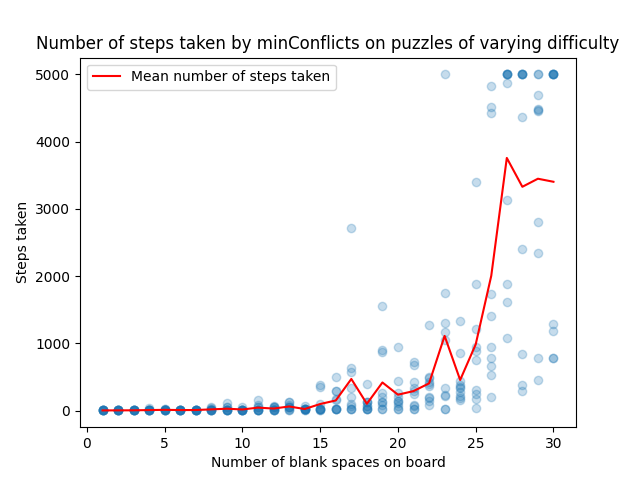
\includegraphics[height=3.65in]{figure1.png}
	\caption{the average number of steps taken by \textit{minConflicts} across the boards.}
	\end{figure}
	
	For \textit{backtrackingSearch}, I measured the time it took for the algorithm to reach a solution for each board. Figure 2 shows the distribution of solve times for backtracking search across the boards. According to the plot, backtracking performs very well for most board difficulties. As complexity increases, backtracking may take more time on some puzzles than others, but the median solve time is no more than a few seconds for even the hardest of puzzles.
	
	\begin{figure}[h]
	\centering
	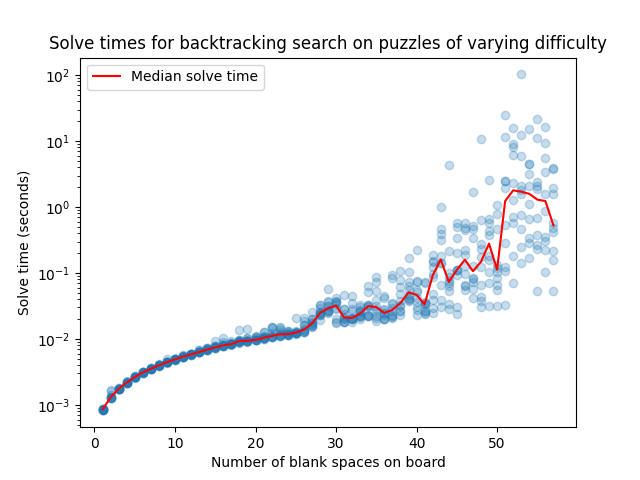
\includegraphics[height=3.65in]{figure2.png}
	\caption{the solve times for \textit{backtrackingSearch} across the boards.}
	\end{figure}
	
	Figure 3 shows the distribution of solve times for \textit{constraintProp}. It turns out that backtracking with constraint propagation performs dramatically better than regular backtracking search. According to the plot, the median solve time for even the hardest puzzles is about 0.05 seconds. 
	
	\begin{figure}[h]
	\centering
	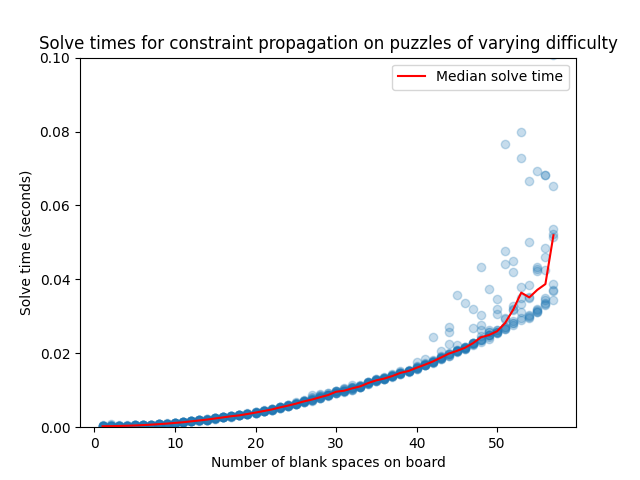
\includegraphics[height=3.65in]{figure3.png}
	\caption{the solve times for \textit{constraintProp} across the boards.}
	\end{figure}
	
	\begin{figure}[h]
	\centering
	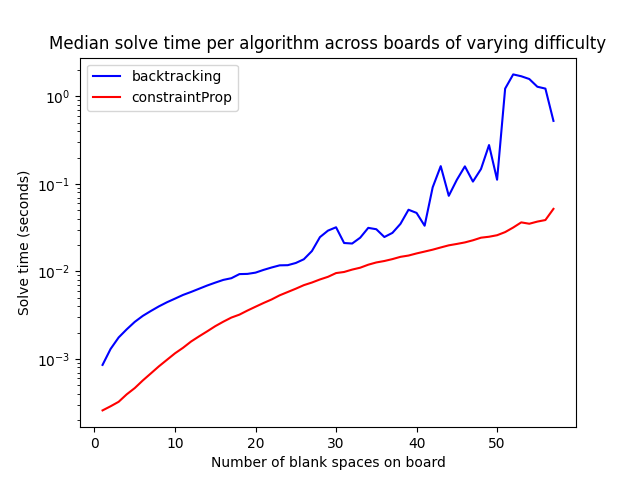
\includegraphics[height=3.65in]{figure4.png}
	\caption{the median solve times for \textit{backtrackingSearch} and \textit{constraintProp} across the boards.}
	\end{figure}\\
	
	If we plot the median solve times for \textit{backtrackingSearch} and \textit{constraintProp} against one another, as in Figure 4, we can see just how much better \textit{constraintProp} performs.\\\\
	\textbf{Analysis}

	The results are in: \textit{minConflicts} comes in third, \textit{backtrackingSearch} takes second, and \textit{constraintProp} is our champion. But why is this the case? Recall that \textit{minConflicts} relies on random choice to set values. As the number of blank cells increases, the number of possible complete assignments to a board increases exponentially. Even if \textit{minConflicts} iterated over random assignments, it would take exponentially longer to find the solution to a board of increasing complexity. But since the initial assignment is random, more empty spaces means more opportunities for the algorithm to plateau, reset, and reiterate. Perhaps a dynamic plateau threshold---one that increases with the complexity of the input board---would result in better performance; but there are clearly better algorithms out there.
	
	Backtracking is an efficient approach, but it is not well-suited for some boards. Recall that general backtracking chooses the first empty cell in order of its appearance on the board---that is, top-down and left-to-right. General backtracking uses depth-first search and prunes trees that result in conflicts. If a board's blank spaces are oriented such that backtracking does not encounter conflicts until deep within its search tree, the algorithm may take longer to find a solution. Let's refer to a board oriented this way as a `fluke'. More blank spaces on a board means that that board is more likely to be a fluke and trick the backtracking algorithm. This explains why in Figure 2, after 50 or so blank spaces, backtracking search's performance begins to vary more.
	
	\textit{constraintProp} seems to largely escape this by choosing the empty cell that has the least possible candidates. It is faster overall than general backtracking because it only tests values over a cell's candidates, which automatically prunes large branches of the search tree. This is expected as \textit{constraintProp} is a specialized adaptation of \textit{backtrackingSearch}. It's worth noting that \textit{constraintProp} mirrors a common human approach to Sudoku by keeping track of the possible values for each cell. In fact, the NYT Games app has a mode that allows the player to note down candidates for each cell!
	
	So, which algorithm is best? If the board has only a few blank spaces, any algorithm will do well. But if you're trying to outsmart the conniving puzzle-writers at the New York Times, your best bet is a backtracking approach using constraint propagation and the Minimum Remaining Values heuristic. Happy solving!
	
\newpage
\begin{center}
	\textbf{References}
\end{center}
\begin{list}{}{ 
    \setlength{\itemindent}{-0.5in}
    \setlength{\leftmargin}{0.5in}
    }
\item Russell, S., and Norvig, P. (2009). \textit{Artificial Intelligence: A Modern Approach} (3rd ed.). Pearson.
\item The New York Times. (n.d.). \textit{Play Sudoku}. The New York Times. https://www.nytimes.com/ puzzles/sudoku
\end{list}
The code for this project can be found in the following GitHub repository:
\begin{center}
	https://github.com/arjunphull123/sudoku-ai
\end{center}
\end{document}
